\section{\LARGE{Utilizzo delle colture cellulari umane in analisi molecolari e morfologiche}}

\vspace{0.6cm}

\subsection{Sommario}

\subsubsection{Scopo}

In questa esperienza sono state utilizzate delle colture cellulari
di melanoma umano.
Queste colture saranno usate per la raccolta dell'RNA e l'analisi proteica.
Una terza coltura è stata colorata con un colorante viola per poter
osservare al microscopio le cellule.

\subsubsection{Cenni teorici}

Le colture cellulari sono molto importanti per poter studiare le cellule durante
il loro ciclo vitale, e per amplificare DNA, RNA e proteine semplificandone l'estrazione.

\subsubsection{Strumenti e materiali utilizzati}

\begin{itemize}
\item Guanti in lattice
\item Pasteur in plastica monouso
\item Cell scraper
\item Falcon da utilizzare come scarto
\item Provette Eppendorf (2mL)
\item Micropipette (\SI{100}{\micro\liter}-\SI{1000}{\micro\liter} e \SI{2}{\micro\liter}-\SI{200}{\micro\liter})
\item Microscopio ottico
\end{itemize}

\subsubsection{Soluzioni utilizzate}

\begin{itemize}
\item Cristalvioletto in eppendorf da 1,5ml
\item RNAlater in eppendorf da 1,5ml
\item 5ml PBS 10X + 45ml ddH$_2$O, in provetta Falcon 50ml
\end{itemize}

\subsection{Procedimento}

\subsubsection{Raccolta cellule per analisi proteica}

\begin{enumerate}

\item Aspirare completamente il terreno di coltura con la pasteur.
\item Aggiungere con la pasteur 1ml di PBS, riaspirarlo con quest'ultima e scartarlo.
\item Ripetere la procedura precedente.
\item Aggiungere 1,5ml di PBS.
\item Staccare le cellule con il cell scraper.
Dopo averlo utilizzato lo conserviamo nel fodero per riutilizzarlo successivamente
Per staccare le cellule con questo strumento, muovere esercitando una leggera pressione
e spostarsi lungo tutta la superficie.
\item Aspirare 1,5ml di PBS con le cellule in sospensione e trasferire su una eppendorf da 2ml
\item Centrifugare per 10 minuti a 10000g.
\item Adesso tutte le cellule si trovano sul fondo formando un pellet. Aspirare tutto
i PBS sopranatante facendo attenzione a non staccare il pellet.
\item Conservare a -20°C per la successiva estrazione delle proteine.

\end{enumerate}

\subsubsection{Raccolta cellule per raccolta RNA}

\begin{enumerate}
    \item Aspirare completamente il terreno di coltura con la pasteur.
    \item Aggiungere con la pasteur 1ml di PBS, riaspirarlo con quest'ultima e scartarlo.
    \item Ripetere la procedura precedente.
    \item Aggiungere 1ml di RNAlater.
    \item Staccare le cellule con il cell scraper.
    \item Aspirare tutto l'RNAlater con le cellule in sospensione e portarlo su una
    eppendorf da 2ml.
    \item Centrifugare per 10 minuti a 10000g.
    \item Adesso tutte le cellule si trovano sul fondo formando un pellet. Aspirare tutto
    i PBS sopranatante facendo attenzione a non staccare il pellet.
    \item Conservare a -20°C per la successiva estrazione degli acidi nucleici.
\end{enumerate}

\subsubsection{Colorazione del tappeto cellulare}

\begin{enumerate}
    \item Aggiungere sotto cappa chimica 1ml di formalina al pozzetto delle cellule da
    colorare e lasciare agire per 20/30 minuti.
    \item Spostarsi sul bancone e aspirare tutto il liquido con la pasteur e scartarlo.
    \item Aggiungere 1ml di PBS con la pasteur, riaspirarlo con quest'ultima e scartarlo.
    \item Ripetere la procedura con il PBS.
    \item Aggiungere con la pasteur tutto il cristalvioletto contenuto nell'aliquota fornita
    (1ml) facendo attenzione a non sporcarsi.
    \item Lasciare agire il colorante per 30 minuti, dopodich\`e aspirarlo e scartare il colorante.
    \item Aggiungere 1ml di PBS con la pasteur, aspirarlo con quest'ultima e scartarlo.
    \item Ripetere questa procedura altre 3/4 volte per lavare il colorante e poterle visualizzare
    al microscopio.
    \item Aggiungere 1ml di PBS nel pozzetto colorato, ora si possono osservare al
    microscopio le cellule colorate.
\end{enumerate}

\subsection{Risultati e Conclusioni}

In figura vediamo le cellule di melanoma colorate di viola (le sagome irregolari, normalmente non visibili).
Sono inoltre presenti dei puntini viola che corrispondono a dei vacuoli che si sono colorati.

\begin{figure}[htbp]
	\centering
	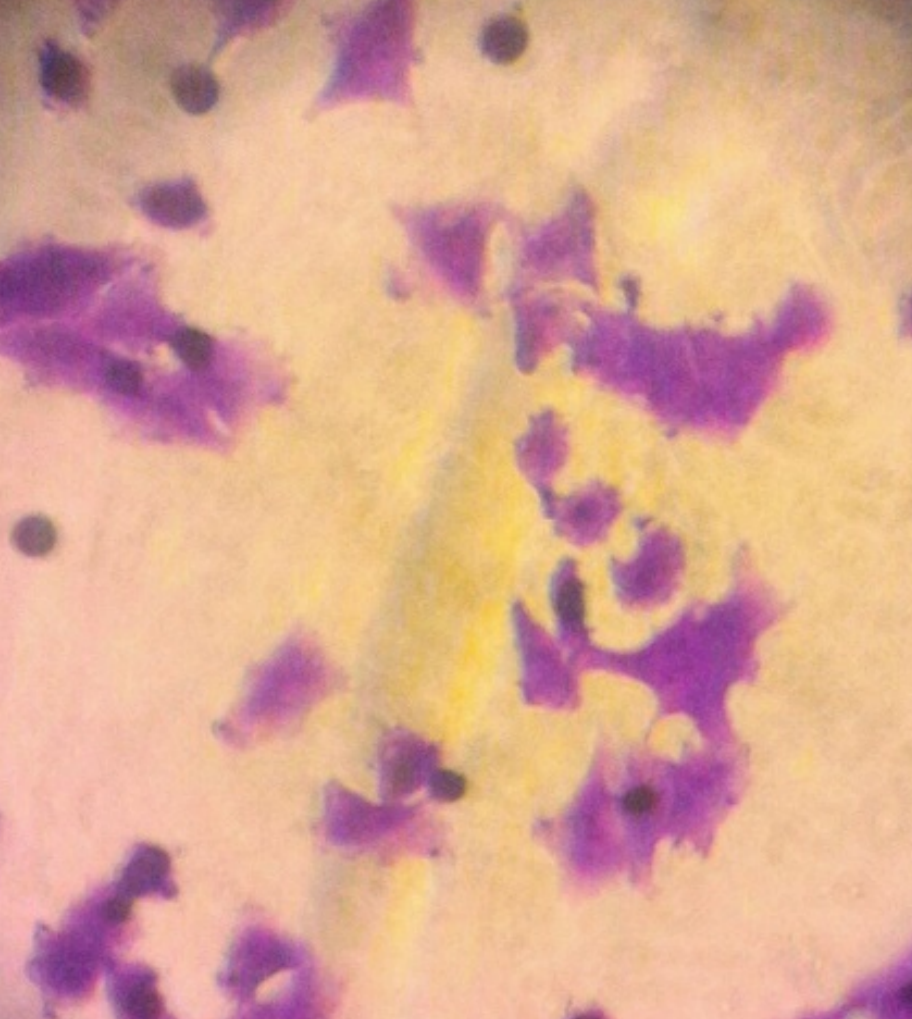
\includegraphics[width=80mm]{./immagini/melanoma.png}
	\caption{Risultati colorazione}
	\label{melanoma}
\end{figure}
